\chapter{基于RBF-SVR的分片逼近模型在直复营销下广告预算分配中的研究}

% 首先介绍多渠道广告投放资金分配问题使用强化学习研究的现状(没有利用强化学习解决该问题的文献,存在的主要问题:数据量较少,导致值函数估计不准确等问题,收敛速度慢,说明本文采用非参数化建模的原因,非参数化建模又存在什么问题,针对此问题又是如何解决的)
% 介绍深度强化学习
% 介绍本文提出的混合网络模型算法
% “我知道我的广告费有一半浪费了,可是我不知道浪费的是哪一半。”美国费城商人约翰·华纳梅克的这句自嘲式的调侃简直让人抓狂——似乎你绞尽脑汁想出的营销点子就是为了达到一个目的——尽量让广告费被浪费得少一点而已。

\section{直复营销下广告预算分配问题阐述}
本章,首先介绍了在直复营销体系下,基于第三方广告代理商进行广告投放的应用场景及其具体的投放过程。然后,说明了广告投放的目标是追求全渠道的基于ROI的LTV最大化,以此作为选择强化学习解决该问题的依据。最后,介绍了广告投放预算分配场景所具有的三个特点,并针对这些特点来针对性的提出解决方法,以优化强化学习算法,将此作为本章研究的出发点。

\subsection{广告预算分配场景}
美国直复营销协会(American Direct Marketing Association,ADMA)\footnote{http://www.the-dma.org/}将直复营销(Direct Response Marketing)定义为一种市场营销体系,运用一种或几种广告媒介在任何地点产生可以度量的反应或交易。直效营销仅仅属于直复营销中的一种应用场景,它特指不通过第三方,中间人,而直接对客户进行推广和营销,以维持企业与客户的良好关系。但是,在这种场景下需要企业有充足的客户资源和大量的相关客户资料,这对于大部分企业是很难办到的,需要很长时间的积累,特别是在日益激烈的市场竞争环境中,时间就是企业的生命线。于是,为了快速获取用户、推广相关产品、扩大公司的收入,越来越多的企业选择通过第三方广告代理商(Ad-agency)进行广告投放。

广告代理商除了帮助企业进行广告设计与策划以外,还有一部分更重要的工作,就是帮助广告主安排或代为购买媒介空间或时间。近年来,随着广告市场的不断发展和扩大,为了方便广告主高效的进行广告投放,大部分在线的广告代理商也都建设了自己的广告投放平台,其投放流程如图$\ref{fig:ad_process}$所示。在广告投放平台上,广告代理商(Ad-agency)有很多可供选择的广告渠道(channel)资源,广告主每次需要提供一个广告投放策略,策略的内容包括在哪些渠道上投放广告以及对应投放多少金额的广告费。然后,广告代理商会按照广告主提供的投放策略,将对应的广告量通过各渠道投放给潜在顾客(广告的受众)。在广告投放结束后,广告代理商会将此次广告投放的直观效果反馈给广告主,同时广告主也可以通过追踪已经交易的顾客的后续信息,综合评价此次的投放效果。

\begin{figure}[htbp]
\centering
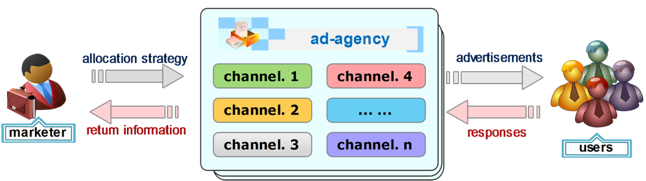
\includegraphics[width=0.8\textwidth]{ad_process}
\caption{基于ad-agence的广告投放过程}
\label{fig:ad_process}
\end{figure}

通过以上的介绍,可以看到在通过广告代理商投放广告的过程中,顾客可以及时接收到广告主发布的广告信息,而广告主也会收到响应顾客的响应反馈,因此广告主与顾客之间是存在互动性的。另外,广告主还可以根据广告代理商反馈的投放效果信息以及追踪用户未来行为等方式去量化此次广告投放对企业的价值,因此效果是可衡量性的,所以,利用广告代理进行广告投放的方式也属于直复营销体系。

在企业进行广告投放的真实业务中,为了保证财务帐面的稳定以及公司合理健康的发展,公司财务每个月都会给出该月的广告投放资金的预算,然后广告投放部门会在此预算下进行广告预算的合理分配,以使得公司的业务不断扩大、收入持续增长。但是,因为广告投放场景比较复杂,单纯靠广告投放人员制定预算分配策略往往很持续难达到好的效果,所以需要充分利用机器学习技术。

\subsection{基于LTV的ROI值}
通常情况下,企业在进行广告投放时,为了达到持久有效的营销效果,而且为了能够更好的评价广告渠道的质量,一般都会在一个广告代理商下进行为期一年或几年的持续投放。因此,广告投放是一个序列化的过程。

评价广告投放效果的重要指标是投资回报比(Return On Investment, ROI)即一定周期内,广告主通过广告投
放收回的价值占广告投入的百分比,计算方法如式\eqref{seq4_1}所示,其中Income表示收入额,Cost表示成本,Investment表示投资额,一般情况下认为Cost和Investment是同一概念。
\begin{equation}
\label{seq4_1}
\begin{aligned}
 ROI=\frac{Income-Cost}{Investment}*100\%
\end{aligned}
\end{equation}

但是,在广告投放的过程中,用户的反馈存在一定的延迟,而且某一时刻的投放的广告会对后面时刻的广告投放效果产生一定程度的影响,所以不能仅仅使用即时的ROI值作为广告效果的评价指标。比如,一个顾客在某一时刻看到该广告,但是并没有立刻产生正向反馈或者交易,而是在经过若干时间后的某一时刻才有正向反馈。那么,此时所产生的收益不单单与现在这个时刻的广告投放效果有关,还与之前的广告投放效果有关。所以,在计算广告投放所产生的回报时,应该要有全局观念。在实际应用中,广告主一般将基于渠道LTV的ROI值作为评价广告渠道质量的指标,在此场景中,LTV是指渠道所产生的累积回报,只要将公式\eqref{seq4_1}中的Income换成渠道的LTV值即可。

通过第二章的介绍,我们知道,强化学习在处理序列问题时,很好的考虑到了延迟奖赏的问题,并且以追求累积奖赏最大化作为优化目标,所以将强化学习技术应用在广告投放领域,可以充分发挥其优势,预期取得较好的结果。

\subsection{广告预算分配特点}
% 多渠道/总预算限制/数据量少
解决好广告投放的资金预算分配问题虽然有着很高的商业价值和现实意义,但是并没有引起很多学者和专家的研究。其中,最主要的原因就是没有在此领域公开的数据集。本文的数据是基于国内某公司在进行广告投放过程中所产生的真实数据,所以研究内容具有的实用性和真实性。

即便拥有了相关的广告投放数据,但是因为还存在诸如场景复杂、数据量少、预算约束等问题,从而影响强化学习的优化效果。本文就是针对这些存在的问题进行分析,并提出了相应的解决方法。

对于大部分企业来说,广告投放是以天为单位进行的,所以投放数据量比较少,严重影响了模型的训练和学习。因此,为了提高数据的使用率,我们考虑使用非参数化函数的逼近方法进行强化学习的训练。另外,一般在广告投放时会选择多个渠道同时进行投放,所以,我们不能只考虑到渠道自身延迟反馈的影响,而且还应该考虑渠道间的相互影响。最后,每一次的广告投放策略都需要在给定的固定预算的约束下进行,所以我们在使用强化学习进行值估计后,还要考虑如何进行预算资金的分配。

\section{SVR-RBF+Q分块逼近模型}
在真实的广告投放场景中,广告主进行广告投放的周期是相对较长的(一天一次),所能得到的数据也相对较少。所以,在进行Q值函数逼近值时,要求我们充分高效的利用仅有的训练样本。然而通过第二章的介绍,我们知道在参数化函数逼近方法中,线性逼近值函数的逼近能力较弱、效率较低,非线性函数(神经网络)逼近又需要有充足的训练样本,所以综合考虑,我们选择了基于非参数化函数逼近的模型,因为该模型是一种基于样本的学习方法,具有较高的灵活性,而且适用于小样本数据。

但是,非参数化函数逼近常常面临着收敛性难移保证的问题。于是,本章提出了基于SVR-RBF+Q的强化学习模型,在该模型中,将对Q值函数逼近问题转化为高维特征空间中的线性回归问题,从而可以加快函数的收敛速度。另外,为了在小数据集下提高函数逼近的精度,提出分块逼近的思想,每个行为作为一块,分别使用SVR-RBF+Q模型进行训练,最后再利用训练好的分块模型多路逼近Q值函数。

\subsection{分块逼近思想}
在广告投放应用中,我们可获得的数据量比较少,如果将所有渠道合在一起进行建模,很难拟合出可靠的值函数变化规律,所以我们采取分渠道进行建模的思路。进一步地,每个渠道在进行值函数的逼近时,考虑到状态空间和行为空间(广告花费)是连续的,如果数据样本较少也会造成状态行为值函数逼近的不准确的后果。

针对以上问题,本章提出分块逼近的思想。离线学习阶段,首先,使用一种花费空间离散化的方法(下文会详细介绍),将花费空间离散为$k$个行为($k$个块)$A=\{a_{1},a_{2},\cdots,a_{k}\}$,然后将训练样本($s_{t},c_{t},r_{t+1},s_{t+1}$)中的花费$c_{t}$转换成相对应的离散行为$a_{t}$,利用Q值函数的更新公式(算法$\ref{algo:algorithm_2}$中第7行)计算Q值,并将Q值添加到对应的样本中($s_{t},a_{t},Q(s_{t},a_{t}),s_{t+1}$)。然后根据行为的不同划分样本,形成$k$个样本单元。接着,利用非参数化逼近模型$M$对样本单元进行建模,$M=\{M_{i}|i=1,2,\cdots,k\}$,每个离散行为对应一个只关于状态的子模型,且各个子模型之间是相互独立。最后,将$k$个子模型合在一起共同逼近Q值函数。每一次迭代过程中,都对所有样本重新更新Q值,直到满足设定的条件。

\subsection{RBF-SVR+Q模型}
假设第$i$个行为对应的样本单元$X_{i}=\{(s_{ij},Q_{ij})\}_{j=1}^{N_{i}}$,其中$s_{ij}$为输入的状态,$Q_{ij}$为输出的Q值,$N_{i}$为样本的个数,我们的目标就是要拟合$s_{ij}$和Q$_{ij}$之间的回归关系。因为数据量少的原因,我们采用的是基于核函数的支持向量回归(Support Vector Regression, SVR)方法来逼近Q值函数,即RBF-SVR+Q模型

在我们的模型中,以结构化风险最小为目标,需要学习一组仿射函数$f_{i}$,$i=1,2,\cdots,k$。即
\begin{equation}
\begin{aligned}
f_{i}=w_{i}^{T} \phi(s) + b_{i}, i=1,2,\cdots,k
\end{aligned}
\end{equation}
式中,$f_{i}$就是我们要学习的Q函数,即$f_{i}=Q_{i}$。$\phi(\cdot)$表示可以将样本从非线性空间映射到高维线性空间的方法,$w_{i}$表示线性回归函数的权值向量,$b_{i}$是一个偏置项。

现仅考虑逼近某一个值函数$Q_{i}$,其共有$N_{i}$个样本,根据SVR的原理,可以将原问题转化为$N_{i}$个带有约束条件的优化问题:
\begin{equation}
% \left\{\begin{matrix}
\begin{aligned}
min_{w_{i},b_{i},\xi_{i},\hat{\xi_{i}}} J_{i}(w_{i},b_{i},\xi_{i},\hat{\xi_{i}}) = \left \| w_{i} \right \|^{2} + C_{i} \sum_{i=1}^{N_{i}}(\xi_{i}+\hat{\xi_{i}})\\ 
s.t \begin{matrix}
 &Q_{ij}-w_{i}^{T} \phi(s_{ij}) - b_{i} \leqslant \epsilon + \xi_{i}\\
 &w_{i}^{T} \phi(s_{ij}) + b_{i} - Q_{ij} \leqslant \epsilon + \hat{\xi_{i}} \\
 &\xi_{i} \geqslant 0,\hat{\xi_{i}} \geqslant 0, j=1,2,\cdots,N_{i}\\
\end{matrix}
\end{aligned}
% \end{matrix}\right.
\end{equation}
% 式中,\xi_{i},\hat{\xi_{i}}为松弛因子,C_{i}是正则化参数,用于控制对超出误差允许范围的样本的惩罚程度,w_{i}为权值向量,用于控制模型的复杂程度。

引入拉格朗日乘子,将原空间的约束优化问题转化为对偶空间的无约束优化问题,得到拉格朗日函数:
\begin{equation}
\begin{aligned}
L_{i}(w_{i},b_{i},\alpha_{i},\hat{\alpha}_{i},\xi_{i},\hat{\xi_{i}},\mu_{i},\hat{\mu}_{i})=&\frac{1}{2} \left \| w_{i} \right \|^{2} + C_{i} \sum_{i=1}^{N_{i}}(\xi_{ij} + \hat{\xi_{ij}}) - \sum_{i=1}^{N_{i}}\mu_{ij}\xi_{ij} - \sum_{i=1}^{N_{i}}\hat{\mu}_{ij}\hat{\xi_{ij}} \\ 
&+ \sum_{i=1}^{N_{i}} \alpha_{ij}(Q_{ij}-w_{i}^{T} \phi(s_{ij}) - b_{i} - \epsilon - \xi_{ij}) \\
&+ \sum_{i=1}^{N_{i}} \hat{\alpha_{ij}}(Q_{ij}-w_{i}^{T} \phi(s_{ij}) - b_{i} - \epsilon - \hat{\xi_{ij}})\\
\end{aligned}
\end{equation}

求偏导:
$\begin{Bmatrix}
\frac{\partial{L_{i}}}{\partial{w_{i}}}=0 \Righttarrow w_{i}=\sum_{i=1}^{N_{i}}(\hat{\alpha_{ij}}-\alpha_{ij})s_{ij}\\ 
\frac{\partial{L_{i}}}{\partial{b_{i}}}=0 \Righttarrow \sum_{i=1}^{N_{i}} \alpha_{ij} = 0
\\ 
\frac{\partial{L_{i}}}{\partial{\xi_{i}}=0 \Righttarrow  C_{i} = \alpha_{ij} + \mu_{ij}
\\ 
\frac{\partial{L_{i}}}{\partial{\hat{\xi_{i}}}=0 \Righttarrow  C_{i} = \hat{\alpha_{ij}} + \hat{\mu_{ij}}
\end{Bmatrix}$




\section{强化学习在多渠道广告投放预算分配中的建模设计}
\subsection{花费空间离散化方法}
\subsection{渠道间投放影响}
\subsection{改进的探索方法}
\subsection{MCKP结合方法}
\subsection{整体架构}